\documentclass[11pt,a4paper,]{article}
\usepackage{lmodern}

\usepackage{amssymb,amsmath}
\usepackage{ifxetex,ifluatex}
\usepackage{fixltx2e} % provides \textsubscript
\ifnum 0\ifxetex 1\fi\ifluatex 1\fi=0 % if pdftex
  \usepackage[T1]{fontenc}
  \usepackage[utf8]{inputenc}
\else % if luatex or xelatex
  \usepackage{unicode-math}
  \defaultfontfeatures{Ligatures=TeX,Scale=MatchLowercase}
\fi
% use upquote if available, for straight quotes in verbatim environments
\IfFileExists{upquote.sty}{\usepackage{upquote}}{}
% use microtype if available
\IfFileExists{microtype.sty}{%
\usepackage[]{microtype}
\UseMicrotypeSet[protrusion]{basicmath} % disable protrusion for tt fonts
}{}
\PassOptionsToPackage{hyphens}{url} % url is loaded by hyperref
\usepackage[unicode=true]{hyperref}
\hypersetup{
            pdftitle={Assignment 1: Worley},
            pdfborder={0 0 0},
            breaklinks=true}
\urlstyle{same}  % don't use monospace font for urls
\usepackage{geometry}
\geometry{a4paper, centering, text={16cm,24cm}}
\usepackage[style=authoryear-comp,]{biblatex}
\addbibresource{references.bib}
\addbibresource{packages.bib}
\usepackage{longtable,booktabs}
% Fix footnotes in tables (requires footnote package)
\IfFileExists{footnote.sty}{\usepackage{footnote}\makesavenoteenv{long table}}{}
\IfFileExists{parskip.sty}{%
\usepackage{parskip}
}{% else
\setlength{\parindent}{0pt}
\setlength{\parskip}{6pt plus 2pt minus 1pt}
}
\setlength{\emergencystretch}{3em}  % prevent overfull lines
\providecommand{\tightlist}{%
  \setlength{\itemsep}{0pt}\setlength{\parskip}{0pt}}
\setcounter{secnumdepth}{5}

% set default figure placement to htbp
\makeatletter
\def\fps@figure{htbp}
\makeatother


\title{Assignment 1: Worley}
\providecommand{\subtitle}[1]{}
\subtitle{BEX5200 Climate Change and Carbon Management Strategies}

%% MONASH STUFF

%% CAPTIONS
\RequirePackage{caption}
\DeclareCaptionStyle{italic}[justification=centering]
 {labelfont={bf},textfont={it},labelsep=colon}
\captionsetup[figure]{style=italic,format=hang,singlelinecheck=true}
\captionsetup[table]{style=italic,format=hang,singlelinecheck=true}


%% FONT
\RequirePackage{bera}
\RequirePackage[charter,expert,sfscaled]{mathdesign}
\RequirePackage{fontawesome}

%% HEADERS AND FOOTERS
\RequirePackage{fancyhdr}
\pagestyle{fancy}
\rfoot{\Large\sffamily\raisebox{-0.1cm}{\textbf{\thepage}}}
\makeatletter
\lhead{\textsf{\expandafter{\@title}}}
\makeatother
\rhead{}
\cfoot{}
\setlength{\headheight}{15pt}
\renewcommand{\headrulewidth}{0.4pt}
\renewcommand{\footrulewidth}{0.4pt}
\fancypagestyle{plain}{%
\fancyhf{} % clear all header and footer fields
\fancyfoot[C]{\sffamily\thepage} % except the center
\renewcommand{\headrulewidth}{0pt}
\renewcommand{\footrulewidth}{0pt}}

%% MATHS
\RequirePackage{bm,amsmath}
\allowdisplaybreaks

%% GRAPHICS
\RequirePackage{graphicx}
\setcounter{topnumber}{2}
\setcounter{bottomnumber}{2}
\setcounter{totalnumber}{4}
\renewcommand{\topfraction}{0.85}
\renewcommand{\bottomfraction}{0.85}
\renewcommand{\textfraction}{0.15}
\renewcommand{\floatpagefraction}{0.8}


%\RequirePackage[section]{placeins}

%% SECTION TITLES


%% SECTION TITLES (NEW: Changing sections and subsections color)
\RequirePackage[compact,sf,bf]{titlesec}
\titleformat*{\section}{\Large\sf\bfseries\color[rgb]{0.8, 0.7, 0.1 }}
\titleformat*{\subsection}{\large\sf\bfseries\color[rgb]{0.8, 0.7, 0.1 }}
\titleformat*{\subsubsection}{\sf\bfseries\color[rgb]{0.8, 0.7, 0.1 }}
\titlespacing{\section}{0pt}{2ex}{.5ex}
\titlespacing{\subsection}{0pt}{1.5ex}{0ex}
\titlespacing{\subsubsection}{0pt}{.5ex}{0ex}


%% TITLE PAGE
\def\Date{\number\day}
\def\Month{\ifcase\month\or
 January\or February\or March\or April\or May\or June\or
 July\or August\or September\or October\or November\or December\fi}
\def\Year{\number\year}

%% LINE AND PAGE BREAKING
\sloppy
\clubpenalty = 10000
\widowpenalty = 10000
\brokenpenalty = 10000
\RequirePackage{microtype}

%% PARAGRAPH BREAKS
\setlength{\parskip}{1.4ex}
\setlength{\parindent}{0em}

%% HYPERLINKS
\RequirePackage{xcolor} % Needed for links
\definecolor{darkblue}{rgb}{0,0,.6}
\RequirePackage{url}

\makeatletter
\@ifpackageloaded{hyperref}{}{\RequirePackage{hyperref}}
\makeatother
\hypersetup{
     citecolor=0 0 0,
     breaklinks=true,
     bookmarksopen=true,
     bookmarksnumbered=true,
     linkcolor=darkblue,
     urlcolor=blue,
     citecolor=darkblue,
     colorlinks=true}

\usepackage[showonlyrefs]{mathtools}
\usepackage[no-weekday]{eukdate}

%% BIBLIOGRAPHY

\makeatletter
\@ifpackageloaded{biblatex}{}{\usepackage[style=authoryear-comp, backend=biber, natbib=true]{biblatex}}
\makeatother
\ExecuteBibliographyOptions{bibencoding=utf8,minnames=1,maxnames=3, maxbibnames=99,dashed=false,terseinits=true,giveninits=true,uniquename=false,uniquelist=false,doi=false, isbn=false,url=true,sortcites=false}

\DeclareFieldFormat{url}{\texttt{\url{#1}}}
\DeclareFieldFormat[article]{pages}{#1}
\DeclareFieldFormat[inproceedings]{pages}{\lowercase{pp.}#1}
\DeclareFieldFormat[incollection]{pages}{\lowercase{pp.}#1}
\DeclareFieldFormat[article]{volume}{\mkbibbold{#1}}
\DeclareFieldFormat[article]{number}{\mkbibparens{#1}}
\DeclareFieldFormat[article]{title}{\MakeCapital{#1}}
\DeclareFieldFormat[article]{url}{}
%\DeclareFieldFormat[book]{url}{}
%\DeclareFieldFormat[inbook]{url}{}
%\DeclareFieldFormat[incollection]{url}{}
%\DeclareFieldFormat[inproceedings]{url}{}
\DeclareFieldFormat[inproceedings]{title}{#1}
\DeclareFieldFormat{shorthandwidth}{#1}
%\DeclareFieldFormat{extrayear}{}
% No dot before number of articles
\usepackage{xpatch}
\xpatchbibmacro{volume+number+eid}{\setunit*{\adddot}}{}{}{}
% Remove In: for an article.
\renewbibmacro{in:}{%
  \ifentrytype{article}{}{%
  \printtext{\bibstring{in}\intitlepunct}}}

\AtEveryBibitem{\clearfield{month}}
\AtEveryCitekey{\clearfield{month}}

\makeatletter
\DeclareDelimFormat[cbx@textcite]{nameyeardelim}{\addspace}
\makeatother

\author{\sf\Large\textbf{ Mohammed Faizan}\\ {\sf\large MBAt\\[0.5cm]}}

\date{\sf\Date~\Month~\Year}
\makeatletter
\lfoot{\sf Faizan: \@date}
\makeatother


%%%% PAGE STYLE FOR FRONT PAGE OF REPORTS

\makeatletter
\def\organization#1{\gdef\@organization{#1}}
\def\telephone#1{\gdef\@telephone{#1}}
\def\email#1{\gdef\@email{#1}}
\makeatother
  \organization{Monash University}

  \def\name{Our consultancy - Star Wars\newline Mohammed Faizan}

  \telephone{(03) 9905 2478}

  \email{questions@company.com}                 %NEW: New email addresss

\def\webaddress{\url{http://company.com/stats/consulting/}} %NEW: URl
\def\abn{12 377 614 630}                                    % NEW: ABN
\def\logo{\includegraphics[width=6cm]{Figures/logo}}  %NEW: Changing logo
\def\extraspace{\vspace*{1.6cm}}
\makeatletter
\def\contactdetails{\faicon{phone} & \@telephone \\
                    \faicon{envelope} & \@email}
\makeatother

%%%% FRONT PAGE OF REPORTS

\def\reporttype{Report for}

\long\def\front#1#2#3{
\newpage
\begin{singlespacing}
\thispagestyle{empty}
\vspace*{-1.4cm}
\hspace*{-1.4cm}
\hbox to 16cm{
  \hbox to 6.5cm{\vbox to 14cm{\vbox to 25cm{
    \logo
    \vfill
    \parbox{6.3cm}{\raggedright
      \sf\color[rgb]{0.8, 0.7, 0.1 }    % NEW color 
      {\large\textbf{\name}}\par
      \vspace{.7cm}
      \tabcolsep=0.12cm\sf\small
      \begin{tabular}{@{}ll@{}}\contactdetails
      \end{tabular}
      \vspace*{0.3cm}\par
      ABN: \abn\par
    }
  }\vss}\hss}
  \hspace*{0.2cm}
  \hbox to 1cm{\vbox to 14cm{\rule{4pt}{26.8cm}\vss}\hss\hfill}  %NEW: Thicker line
  \hbox to 10cm{\vbox to 14cm{\vbox to 25cm{   
      \vspace*{3cm}\sf\raggedright
      \parbox{11cm}{\sf\raggedright\baselineskip=1.2cm
         \fontsize{24.88}{30}\color[rgb]{0, 0.29, 0.55}\sf\textbf{#1}}   % NEW: title color blue
      \par
      \vfill
      \large
      \vbox{\parskip=0.8cm #2}\par
      \vspace*{2cm}\par
      \reporttype\\[0.3cm]
      \hbox{#3}%\\[2cm]\
      \vspace*{1cm}
      {\large\sf\textbf{\Date~\Month~\Year}}
   }\vss}
  }}
\end{singlespacing}
\newpage
}

\makeatletter
\def\titlepage{\front{\expandafter{\@title}}{\@author}{\@organization}}
\makeatother

\usepackage{setspace}
\setstretch{1.5}

%% Any special functions or other packages can be loaded here.
\AtBeginDocument{\addtocontents{toc}{\protect\thispagestyle{empty}}} 
\usepackage{capt-of}
\usepackage{graphicx}
\usepackage{url}
\usepackage{float}
\usepackage{booktabs}
\usepackage{longtable}
\usepackage{array}
\usepackage{multirow}
\usepackage{wrapfig}
\usepackage{float}
\usepackage{colortbl}
\usepackage{pdflscape}
\usepackage{tabu}
\usepackage{threeparttable}
\usepackage{threeparttablex}
\usepackage[normalem]{ulem}
\usepackage{makecell}
\usepackage{xcolor}


\begin{document}
\titlepage

{
\setcounter{tocdepth}{2}
\tableofcontents
}
``Holding the increase in the global average temperature to well below 2°C above pre- industrial levels and pursuing efforts to limit the temperature increase to 1.5°C above pre- industrial levels, recognizing that this would significantly reduce the risks and impacts of climate change'' (UNFCCC, 2015, pg. 3).

The forces of change, climate change, the energy transition, the increasing importance of the circular economy, and digitalization of industries have compelled establishments to reform and develop sustainable operations. Energy, oil and gas industries are the sectors where this change is felt more rapidly. Worley, is a leading global provider of professional services headquartered in Australia, delivering project and asset services in the energy, chemicals and resources sectors around the world (\textcite{sustainabilityreport2020}). This report explores the climate action and sustainable developments made by Worley and the significance of these commitments in the context of climate change, business motives and the risks and opportunities associated with it.

Worley prides itself with a worldwide network of over 48,000 consultants, engineers, construction workers and data scientists coming together to solve the complexity of the energy, chemicals and resources sectors including turnkey projects that cover the full life-cycle from creating, sustaining and enhancing assets right through to decommissioning and rehabilitation for a sustained economic, social and environmental progress for communities across the world. Worley is committed to Business Ambition for 1.5 through SCIENCE BASED TARGETS INITIATIVE to meet a low carbon future and strive to manage our actions to reduce our emissions and waste. The company has committed to report its performance annually through the sustainability report.

\textbf{Worley is committed to achieving net zero Scope 1 and Scope 2 greenhouse gas emissions by 2030, and to pro-actively supporting our customers to reduce emissions on their projects and assets. We will keep our stakeholders informed of our strategy and progress against established metrics, including the recommendations of the Task Force on Climate-related Financial Disclosure.} \href{https://www.worley.com/sustainability/environment/climate-change}{1}

Our CCPS is supported by a set of strategic actions to help us achieve our ambitions.

\begin{itemize}
\tightlist
\item
  Develop a net zero road map for our Scope 1 and Scope 2 emissions
\item
  Review our Scope 3 emissions and develop a plan to reduce these
\item
  Help our customers to reduce their emissions using our Sustainable Solutions process
\item
  Assess our involvement in carbon-intensive projects using our Responsible Business Assessment Standard
\item
  Report our progress in line with the recommendations of the Task Force on Climate-related Financial Disclosures.
\end{itemize}

\begin{figure}

{\centering 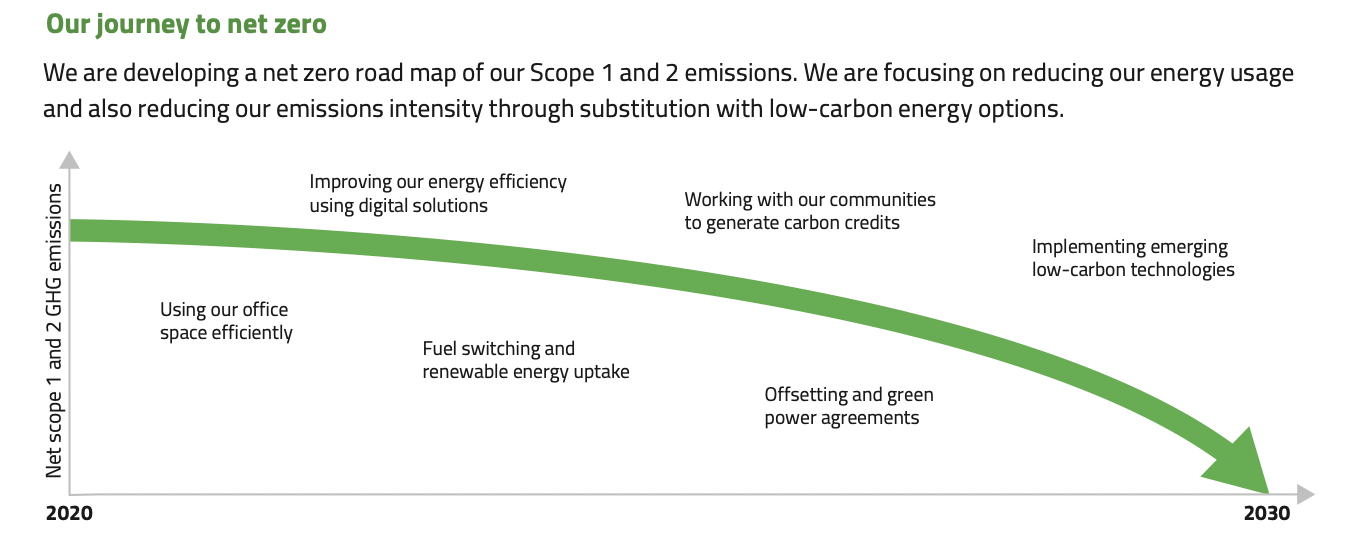
\includegraphics[width=0.5\linewidth]{/Users/mohammedfaizan/git/bex5200/assignment1/BEX5200_Assignment1/Figures/roadmap} 

}

\caption{Road Map towards Net Zero by 2030}\label{fig:roadmap}
\end{figure}

Worley is dependent heavily on its clients as it delivers turnkey projects in across all sectors of energy and chemicals. Climate commitments become significant as there is dependency involved. Worley must be part of brown field projects based on the needs of the client and the project. it is therfore only apt for Worley to commit to Business Ambition for 1.5 through SCIENCE BASED TARGETS INITIATIVE, to scientifically evolve sustainable operations through emission reduction and energy transition. Worley aids its customers who are under pressure to deliver, develop, digitize and decarbonize. The aims of the commitment are in alignment with the Paris Agreement, to achieve net zero by 2050 for its scope 3 emissions. In addition, it promotes Circular Economy, to repurpose goods or recycle them into something else.

The CEO of Worley, Mr.~, realises the significance of Worley's role in the achievement of the Paris Agreement and Sustainable Economic Growth.
``Our commitment to the United Nations Global Compact principles remains as strong as it was 11 years ago when we first signed on.
We released our revised Climate Change Position Statement during the year. It clearly states our ambitions and is supported by strategic actions to help achieve them.'' - CEO, Worley

Climate change affects business and life in unanticipated ways from the temperatures we experience and the availability of drinking water to the habitability of land and the frequency and intensity of extreme weather events. With the growing population, a 10\% increase in energy demand is projected by 2030. These impacts have led government, organisations and businesses to embed climate policies and comply with the Paris agreement. Worley's customers range from oil and gas, power, Refining and Chemicals to Mining, Minerals \& Metals and hence the motive for energy transition, circular economy and other science based target initiatives present a business opportunity for Worley at the same time fulfilling its commitments. Worley has accepted change and thus is more inclined towards sustainable growth of the environment and the communities in which they operate.

Provide examples here.

Worley recognises climate change action, energy transition and supporting customers towards a low-carbon future as key elements of their business strategy

Responding to climate change and the energy transition and supporting, customers towards a low-carbon future are key elements in our business strategy. Risk and opportunities are identified in the market for the company to capitalise on the oppourtinties in energy transition and to mitigate riskd associated associated with declining industries as the world transitions. Worley uses the International Energy Agency Sustainable Development Scenario for strategic planning and develops business resiliency pathways accordingly across its portfolio of businesses and geographies. And their R3 group support businesses in response to physical risks such as extreme weather and rising temperature.

Worley is already investing in renewable energy technology, which is transforming the power sector at an unprecedented rate and designing future-ready infrastructure that can adapt to uses like green hydrogen production. This inherently causes increased attention to deliver future economic returns and to optimise performance and operational cost of existing assets to ensure their competency ahead. The significant cost reduction by use of renewable energy(solar and wind), and distributed power generation systems have motivated the shift from fossil fuels. Dr Paul Ebert, Worley Group Vice President New Energy \& Networks says, ``We are working on projects that allow even larger offshore wind farms to integrate into our current and future energy systems. This includes massive projects that generate both electricity and green hydrogen. Green hydrogen can be used to store energy and then can be used to decarbonize difficult to abate industries.''

Clean energy sector is growing significantly with an estimated 418 GW of offshore wind projects to be installed globally by 2040. This equates to the installation of around 80,000 wind turbines.\emph{Digital technologies} enable companies to be more efficient, to manage energy demand better, store energy, and despatch energy as and when it is required.Worley is ``working on gray, blue and green hydrogen projects all over the world, from studies on the feasibility of crude oil to hydrogen pathways in the Middle East to a detailed study of green hydrogen to ammonia in Australia, and the engineering, procurement and construction of a green hydrogen refueling station in New Zealand.''

Cost reduction in Hydrogen Production (Business Motive): The collaboration with Queensland Nitrates (QNP) and Neoen in Queesnsland to complete a feasibility study to determine commercial production of green hydrogen for its largest use domestic and internationally, ammonia production. The proposed plant would produce 20\% of the ammonia used by QNP which is currently purchased from third parties. Worley is working on digital business models, VECKTA,to optimize Distributed Energy System(DES) with XENDEE. VECKTA is a virtual marketplace for people and companies for the design, technology and sales of DES. Natural gas will play a key role until the mid 2020s in fuel switching and is a bridge to decarbinised energy supply. And, Worley aims to develop projects ``enable communities to develop economically via productive use of natural resources, skills development and lifting communities out of energy poverty'' in the energy, chemicals and resources sectors internationally.

The key performance indicators for Worley's climate commitments include Net zero road map, Worley Foundation, People network groups, Sustainable Solutions process and the TCFD framework for recommendation of the risk, opportunities and progress. The Safe and Sustainable Engineering for Asset Lifecycle (SEAL) framework ensures integrity, safety in design and sustainability and the digital platform, Requis speeeds up procurement process and thereby eliminates waste by using and re-using equipment. As companies race towards net zero, the infrastructure(obselete) plays a vital role in production rate and commodity prices. The Maintenance, Modifications and Operations (MMO) unit of Worley helps its customers to deliver increased productivity in cleaner way, thereby achieving potential project cost. All this progress is reported in Worley's annual Sustainability Report as communication of progress for the UN Global Compact.

\begin{figure}

{\centering 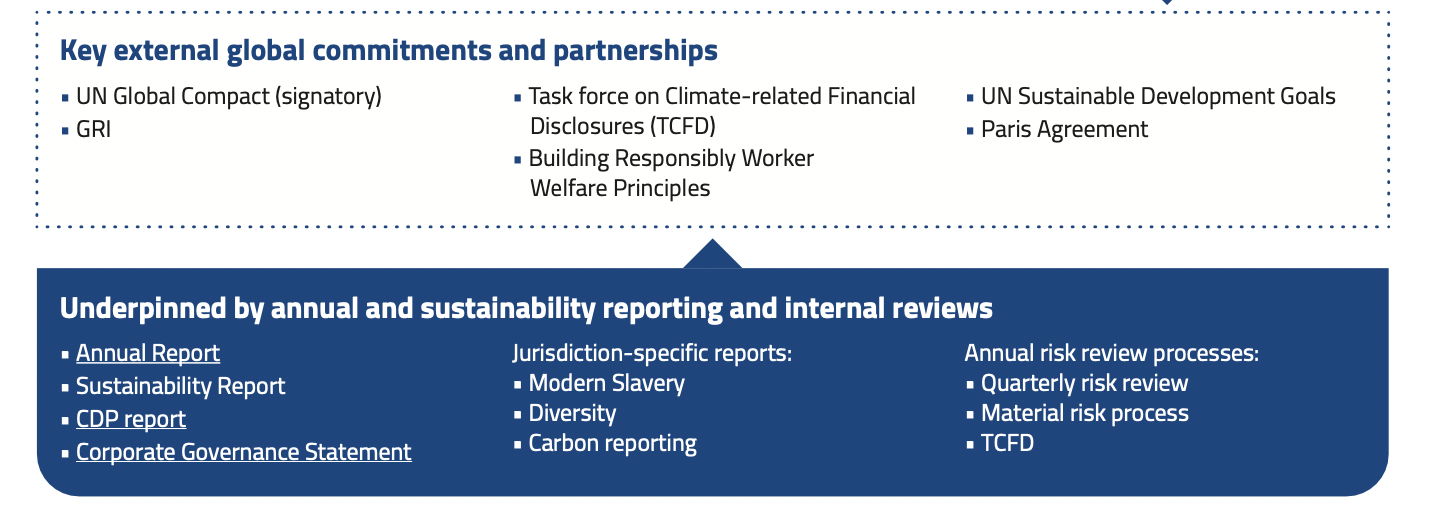
\includegraphics[width=0.5\linewidth]{/Users/mohammedfaizan/git/bex5200/assignment1/BEX5200_Assignment1/Figures/reporting} 

}

\caption{Reporting the Shift}\label{fig:unnamed-chunk-1-1}
\end{figure}
\begin{figure}

{\centering 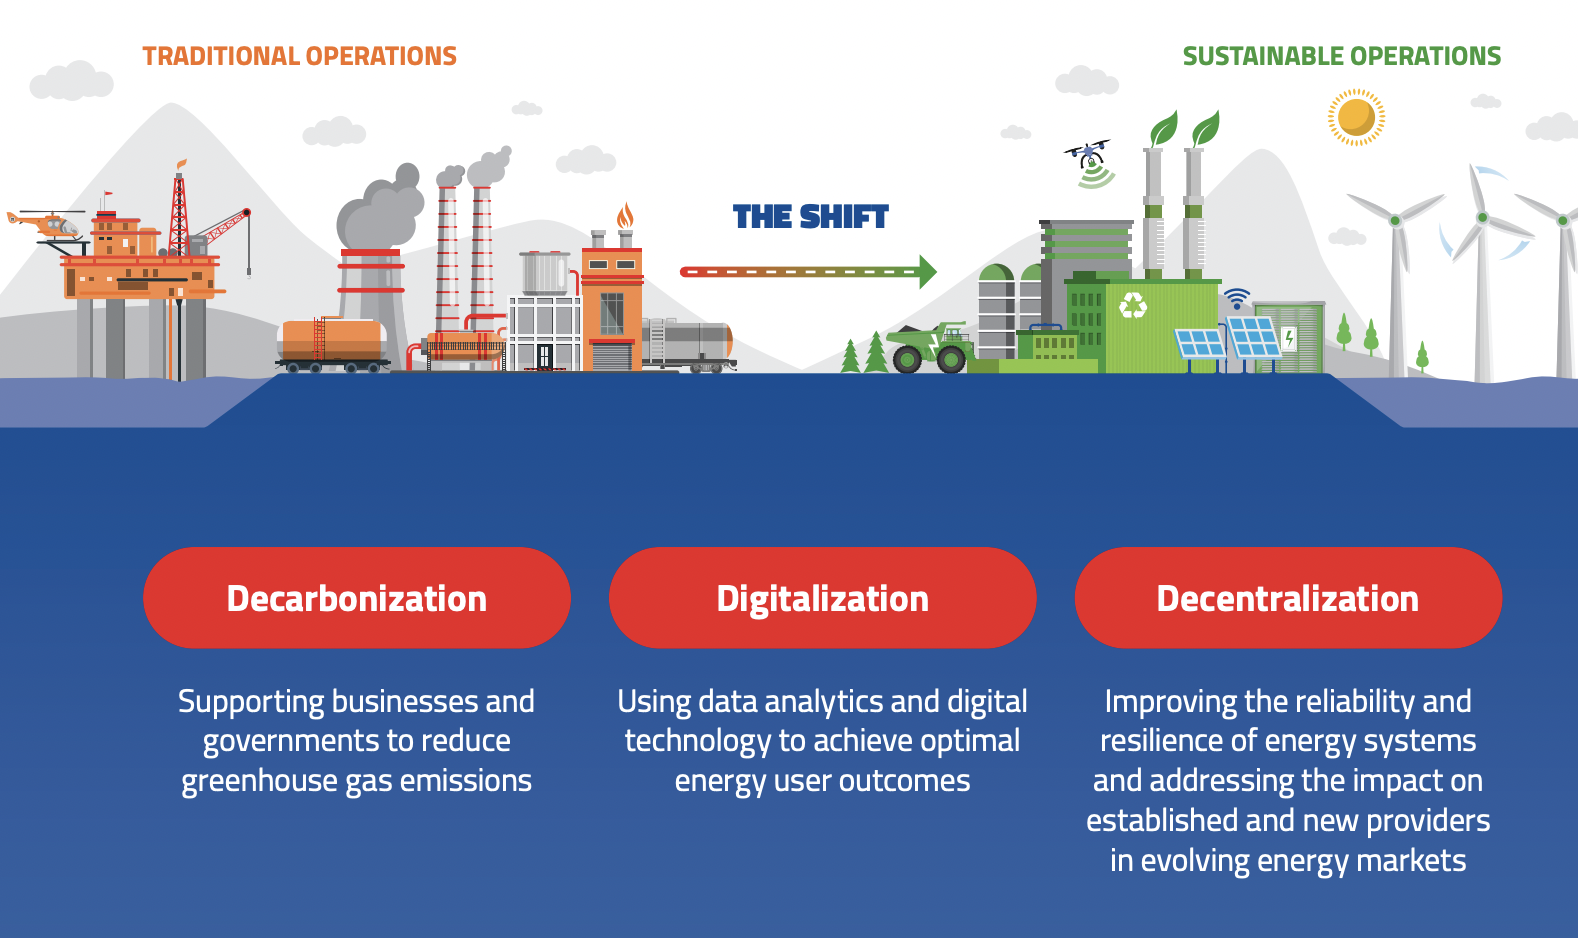
\includegraphics[width=0.5\linewidth]{/Users/mohammedfaizan/git/bex5200/assignment1/BEX5200_Assignment1/Figures/shift} 

}

\caption{Reporting the Shift}\label{fig:unnamed-chunk-1-2}
\end{figure}

``In Australia, we operate around a third of the power generation fleet in the country, across a range of technologies supported by a Remote Monitoring Centre in Sydney.
In the USA, we provide operations and maintenance services to combined cycle, cogeneration and renewable natural gas facilities, including one that uses anaerobic digester technology to produce 4,500+ MMBTU/day of clean, pipeline-quality gas.
In the UK, we helped to install more than 1,250 offshore wind turbines. Through our inspection services, we also helped to maintain over 70\% of offshore turbines - this kept the lights on for the equivalent of 3.15 million UK homes.'' - Worley

What action are they taking? • Have they made progress?
• Are they on track?

To start-off Worley conducted a survey in FY2020 to assess its sustainable growth objectives for its shareholders, customers, internal members and community partners and noted UN's SDG 7: Affordable and clean energy and SDG 13: Climate Action was most favored. Worley claims to support economic growth by creating employment and supporting its customers in their projects. These objectives are being implemented by continued support to customers to navigate the energy transistion, strategic acquisition and joint venture (JV) entities in solar, on-shore and off-shore wind and distributed energy systemsand other projects like providing clean energy to people living in poverty in India with aid from the Pollinate Group.

``In recognition of the importance of sustainable development in the world today, the charter of the Health, Safety and Environment Board committee was expanded this year to include sustainability and is now formally known as the Health, Safety and Sustainability Committee of the Board (Board HSSC).
We are committed to ensuring that Worley has appropriate processes and resources in place to guide the Group's sustainability practices, and that we make relevant disclosures and report performance to our stakeholders.
Worley is committed to being part of the solution through both our own commitments, and also the significant role we can play in supporting the industries we serve.''

The Climate Change Position Statement(CCP) reports the climate commitments and the progress being made and the Sustainable Solutions process overlooks this progress, featuring a carbon calculator, to measure carbon savings; and the Value Creation platform, which captures ideas and reports on those savings, it empowers Worley to identify opportunities to reduce the carbon impact of its customers' projects and to measure savings. The Worley Waste Warriors, a group started in December 2019 to reduce the waste and carbon footprint produced in its offices and improve energy and water efficiency. The Worley Foundation and person donation of Worley employees donated more than \$130,000 to the Red Cross Australian bushfire disaster relief and recovery campaign. ``The Worley Foundation supports scientific research in the Antarctic, Sub Antarctic and Southern Ocean as a Trailblazer10 Corporate Supporter of the Antarctic Science Foundation (ASF)'' to support krill research for the Australian government's Antarctic Division. (reference here). The Worley Foundation, has partnered with Transparency International's (TI) Accountable Mining Program to help identify and address corruption risks in the mining sector, addressing corruption risks in the mining approvals process. The web-based tool by Worley helps TI and supports ethical decision-making in the mining, minerals and metals sectors.

Worley is involved in several clean energy projects across the world. ``Worley is responsible for inspecting more than 70\% of the United Kingdom's offshore wind turbines'',including the world's largest solar project in Dubai. ``Our newest project involves crane, lift and turbine- mounted safety equipment inspection and maintenance services for all 175 3.6 MW turbines at Siemens' London Array offshore wind farm, situated off the south east coast of England. At 630 MW, this wind farm generates enough energy to power more than 470,000 homes and saves the production of over 900,000 tonnes of CO2 every year. That's equivalent to removing emissions from approximately 300,000 cars annually.''

Therefore, Worley is observed from its reports to operate in an environmentally responsible manner considering resource, water and energy efficiency, circular economy principles and environmental impacts. They are believed to contribute project delivery and technical expertise to enable its customers meet the world's changing energy needs in a safe, responsible and sustainable manner, in line with the ambitions of both the Paris Agreement and the United Nations Sustainable Development Goals.

How do your company's commitments compare to similar companies' commitments?
• Would they be in a leadership position within their sector? Are they falling behind their competitors?

\printbibliography

\end{document}
